\documentclass[]{article}
\usepackage{amsmath}
\usepackage{amsthm}
\usepackage{amssymb}
\usepackage[margin=1.3cm]{geometry}
\usepackage{graphicx}
\usepackage{hyperref}

\title{Practical Lab Numerical Computing Computational Finance \\Bachelor-Worksheet 1}
\author{Lukas Troska, Ilja Kalmykov}
\date{}
\setlength{\parindent}{0pt}

\begin{document}
\maketitle 

The source code can be found at \url{https://github.com/iljaGH/CompFin/}.

\section*{Task 1} The program outputs uniformly distributed random
numbers between 0 and 1 in two ways: once by using the C++-function \textit{rand} and
once using the GSL library.

Removing \textit{(double)} in the marked line leads to the result being of type int and thus
either 0 or 1, since division of int by int gives int as the result type in C++.
Thus we have to cast one of the variables to double to force a floating point
division.\\

There is a direct function for simulating normally distributed random variables in GSL.\\
The function \textit{double gsl\_ran\_gaussian(const gsl\_rng* r, double sigma)} returns a
Gaussian random variable with mean 0 and variance sigma.

\section*{Task 2}
Implementation of the rejection sampling algorithm. For code see WS1T32.cpp.

\section*{Task 3} The MATLAB script plots the data against a unit Gaussian
probability density function (PDF). It first creates a histogram of the data, where it
sorts the numbers into 100 different bins and then counts the amount of numbers
in each bin. Then it scales the amount of these numbers to show the relative
amount in each bin and plots it against the unit Gaussian PDF.

The problem in fig. 1 is that $[-2,2]$ is not a good enough bound since the
integral on this interval is $\approx 0.95$. That means we get a lot more variables for which
$y\le p(x')$ (since it is more likely for an element of $[-2,2]$ then say
$[-3,3]$ to fullfill the inequality). Thus the simulated density has a higher mean than the correct density function.

\section*{Task 4} We obtain a normally distributed random variable if we apply the
inverse of the Gaussian cumulative distribution function (CDF) to the uniform random variable.\\
Let $U$ be a standard uniform random variable, $F$ the Gaussian CDF. Then
\[P\left[X\le x\right]=P\left[F^{-1}(U) \le x\right]=P\left[U \le
F(x)\right]=F(x)\]\\
The second equality holds because F is right-continuous; the third
equality holds because U is uniform on [0,1]. This proves the claim.

Intuitively this is clear, too: We uniformly choose a number $U$ between 0 and 1 and
interpret that as a proportion of the area under the Gaussian PDF. Then we
return the $x\in\mathbb{R}$ such that the ratio of the integral of the Gaussian PDF from $-\infty$ to $x$ and the full integral is $U$. Thus,
we are unlikely to choose a number in the tails, since there is little area in
the tails, so we would have to get pick a number very close to 0, whereas for
the other areas the margin is bigger, so we are more likely to return these numbers.

\clearpage
\section*{Task 5} Firstly, the Gaussian CDF is pointsymmetric with respect to the
y-intercept, thus we can handle the case $x<0$ by $1-\mathrm{NormalCDF}(-x)$. If $x>6$,
we know that a standard normally distributed random variable is guaranteed to be smaller,
thus we return 1. For $0\le x\le 1.87$ it's easy to see
that the term given in the return is very close to the Gaussian CDF since
the CDF behaves almost like a polynomial in that area. For the last case the values
of the Gaussian CDF are very close to 1 and, again, like above, the term in the code gives us a
good approximation of the difference of the CDFs value to 1.

\section*{Task 6} Box-Muller method. For code see WS1T36.cpp.
\begin{figure}[!ht]
\centering
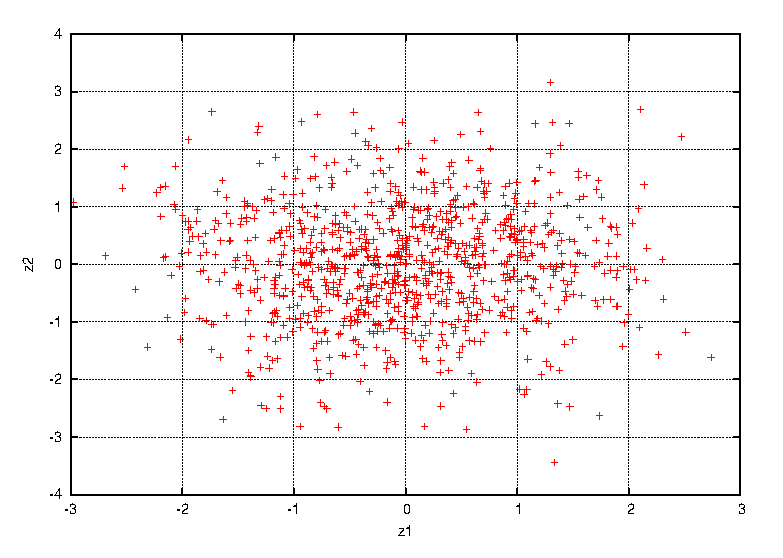
\includegraphics{task6}
\caption{Box-Muller method, 1000 samples}
\label{fig:Task6}
\end{figure}

\section*{Task 7} Let \[g_1(u_1,u_2)=\sqrt{-2\log(u_1)}\cos(2\pi
u_2),\quad g_2(u_1,u_2)=\sqrt{-2\log(u_1)}\sin(2\pi u_2)\] be the transformation
(denoted as $z_1, z_2$ in the problem). Solving for $u_1,u_2$ gives us \[u_1 =
\exp({-(z_1 ^2+ z_2 ^2)/2}),\quad u_2 = (1/2\pi)\tan^{-1} (z_2/z_1).\] The joint
distribution of $z_1, z_2$ is described by \[f(z_1 ,z_2) = f_{u_1,
u_2}(g_1^{-1}(z_1,z_2),g_2^{-1}(z_1,z_2))\cdot| J(g) |\] where $J(g)$ is the
Jacobion matrix of the transformation. Plugging both in we get
\[f(z_1,z_2)=(\exp(-({z_1}^2+{z_2}^2)/2))/(2\pi)=-(\exp(({z_1}^2/2))/\sqrt{2\pi}\cdot\exp(({z_1}^2/2))/\sqrt{2\pi}.\]
We see that $z_1,z_2$ are independent and standard normally distributed.

\clearpage
\section*{Task 8} The advantage of this algorithm is that it is more precise; we
don't have a lot of floating point errors. The variable alpha in the algorithm
is the estimated mean. It is the same as the naive computation: 
\begin{eqnarray}
    \hat{\mu}_n &= &\frac{1}{N}\sum_{i=1}^n x_i\nonumber\\
    &=&\frac{1}{N}\sum_{i=1}^{n-1}x_i+\frac{1}{N}x_n\nonumber\\
    &=&\frac{\hat{\mu}_{n-1}\left(N-1\right)+x_n}{N}\label{eqn:meanAlg}
\end{eqnarray}

and
\begin{eqnarray}
    \hat{\sigma}^{2}_n\left(N-1\right) &= &\sum_{i=1}^n
    \left(x_i-\mu\right)^2\nonumber\\
    &=&\sum_{i=1}^{n-1}\left(x_i-\mu\right)^2
    +\left(x_n-\mu\right)^2\nonumber\\
    &=&\left(N-2\right)\hat{\sigma}^{2}_{n-1} +
    \left(x_n-\mu\right)^2\label{eqn:varAlg}
\end{eqnarray}

Let $x_n$ be the n-th value, $\hat{\mu}_n$ and $\hat{\sigma}_n$ be the n-th
estimated mean value and variance.  For the variables in the
algorithm we have:
\[\gamma=x_n-\hat{\mu}_{n-1},\quad \alpha=\hat{\mu}_{n-1},\quad \beta = \beta +
\gamma^2\frac{n-1}{n},\quad \sigma = \sqrt{\frac{\beta}{n-1}} =
\hat{\sigma}_{n}\]

where $n=i+1$. Obviously $\hat{\mu}_0=x_0$ and $\hat{\sigma}_0 = 0$, so the initialization is
correct. The computation is correct, too, since in the terms above and with
(\ref{eqn:meanAlg}) and (\ref{eqn:varAlg}), we have:
\begin{eqnarray*}
      \alpha & = &\alpha+\gamma/(i+1) \\
      & = &\hat{\mu}_{n-1}+(x_n-\hat{\mu}_{n-1})/n \\
      & = &((n-1)\hat{\mu}_{n-1}+x_n)/n \\
      & = &(x_1+...+x_n)/n = \hat{\mu}_{n}
\end{eqnarray*} 

\begin{eqnarray*}
      \sigma^2 \left(n-1\right) & = & \beta \\
      & = & \beta + \gamma^2\frac{n-1}{n}\\
      & = & \hat{\sigma}^{2}_n\left(n-1\right) + \gamma^2\frac{n-1}{n}\\
      & = & \left(\frac{\hat{\sigma}^{2}_n n+\gamma^2}{n}\right)\left(n-1\right)
      \\
      & = & \hat{\sigma}^{2}_{n+1}\left(n-1\right)
\end{eqnarray*} 

This shows that it yields the same result.
\clearpage
\section*{Task 9}
Estimation of mean and variance of a $\mathcal{N}(\mu,\sigma^2)$-distributed variable, where $\mu$ and $\sigma$ are $\mathcal{U}(0,10)$-distributed. For code see WS1T39.cpp.\\
\begin{figure}[!ht]
\centering
\includegraphics{task9_mu}
\caption{Convergence plot for estimation of $\mu$}
\label{fig:Task9a}
\end{figure}

\begin{figure}[!ht]
\centering
\includegraphics{task9_sigma_mu}
\caption{Convergence plot for estimation of $\sigma$ given $\mu$}
\label{fig:Task9b}
\end{figure}

The error is approximately given by $O(N^{-\frac{1}{2}})$.

\newpage
\section*{Task 10} Simulation of 3 paths of a Wiener process and corresponding asset prices using $S(0)=10,\mu=0.1,\sigma=0.2,T=2$. The paths look more or less the same independent of time discretization, also the mean price change is indeed +10\%/year. For code see WS1T510.cpp.\\


\begin{figure}[!ht]
\centering
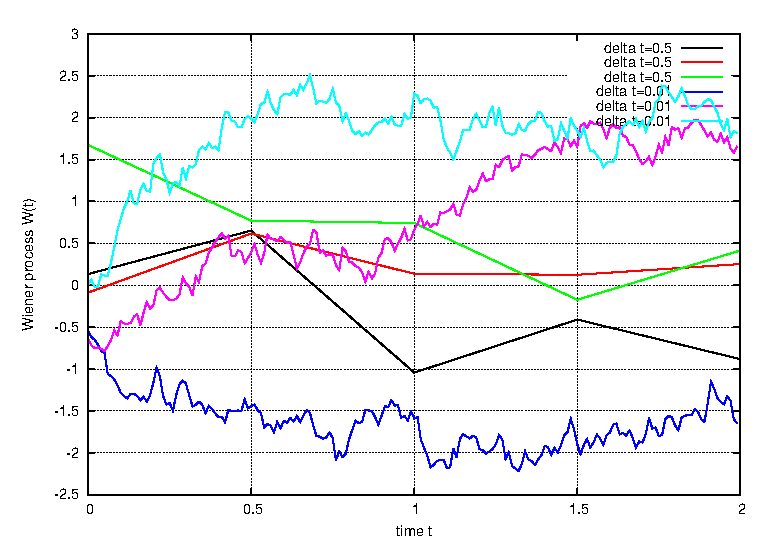
\includegraphics{task10_w}
\caption{Wiener processes with parameters $S(0)=10,\mu=0.1,\sigma=0.2,T=2$}
\label{fig:Task10a}
\end{figure}

\begin{figure}[!ht]
\centering
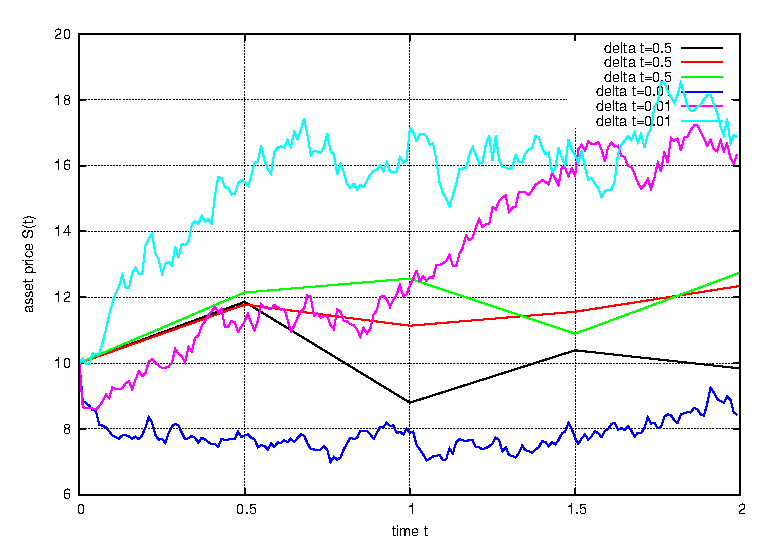
\includegraphics{task10_s}
\caption{Corresponding asset prices}
\label{fig:Task10b}
\end{figure}
\clearpage
\end{document}
